\documentclass[UTF8,zihao=-4]{ctexart}

\usepackage[a4paper,margin=2.35cm]{geometry}
\usepackage{amsmath,amssymb,amsthm,booktabs,array,longtable}
\usepackage{graphicx,float,enumitem,microtype}
\usepackage[font=small,labelfont=bf]{caption}
\usepackage{algorithm,algpseudocode}
\usepackage[table]{xcolor}
\usepackage{tikz}
\usetikzlibrary{arrows.meta,positioning,fit,backgrounds,calc}
\usepackage{titlesec,titletoc,fancyhdr}
\usepackage{hyperref}

\definecolor{coverbg}{RGB}{9,24,42}
\definecolor{coverbg2}{RGB}{13,33,56}
\definecolor{gold}{RGB}{201,162,77}
\definecolor{cyanx}{RGB}{96,186,208}
\definecolor{ink}{RGB}{232,238,245}
\definecolor{muted}{RGB}{138,158,180}
\definecolor{faint}{RGB}{60,84,110}
\definecolor{accent}{RGB}{16,54,92}
\definecolor{rulegold}{RGB}{170,134,56}
\definecolor{graytext}{RGB}{110,122,138}
\definecolor{success}{RGB}{50,115,82}
\definecolor{warning}{RGB}{160,91,49}

\hypersetup{
  colorlinks=true,
  linkcolor=accent,
  citecolor=accent,
  urlcolor=accent,
  pdfauthor={周梓煜、张心湉、许艺馨、张修博、刘迅羽、王佳祺},
  pdftitle={结构化字段之外，文本还剩多少 Alpha？},
}

\setlength{\parindent}{2em}
\setlength{\parskip}{0.25em}
\setlength{\headheight}{16pt}
\renewcommand{\arraystretch}{1.22}
\captionsetup{labelfont={bf,color=accent}}
\captionsetup[table]{skip=5pt}
\captionsetup[figure]{skip=6pt}
\tolerance=2000
\emergencystretch=2.5em

\titleformat{\section}
  {\normalfont\heiti\fontsize{15}{20}\selectfont\color{accent}}
  {\color{rulegold}\thesection}{0.7em}{}
  [{\vspace{2pt}\color{rulegold}\titlerule[0.9pt]}]
\titlespacing*{\section}{0pt}{1.7em}{0.9em}
\titleformat{\subsection}
  {\normalfont\heiti\fontsize{12}{16}\selectfont\color{accent}}
  {\color{rulegold}\thesubsection}{0.6em}{}
\titlespacing*{\subsection}{0pt}{1.2em}{0.55em}

\pagestyle{fancy}
\fancyhf{}
\fancyhead[L]{\small\color{accent}结构化字段之外，文本还剩多少 Alpha？}
\fancyhead[R]{\small\color{graytext}\nouppercase{\leftmark}}
\fancyfoot[C]{\small\color{graytext}\thepage}
\renewcommand{\headrulewidth}{0pt}
\renewcommand{\footrulewidth}{0pt}
\renewcommand{\headrule}{\vspace{2pt}{\color{rulegold}\hrule height 0.7pt}}
\fancypagestyle{plain}{\fancyhf{}\fancyfoot[C]{\small\color{graytext}\thepage}\renewcommand{\headrule}{}}

\titlecontents{section}[0em]
  {\addvspace{7pt}\heiti\color{accent}}
  {\contentslabel{1.7em}}{}
  {\hspace{0.4em}\color{rulegold}\titlerule*[0.7pc]{$\cdot$}\color{accent}\contentspage}
\titlecontents{subsection}[2.1em]
  {\addvspace{2pt}\small\color{black!72}}
  {\contentslabel{2.5em}}{}
  {\hspace{0.4em}\color{black!25}\titlerule*[0.7pc]{$\cdot$}\color{black!72}\contentspage}

\makeatletter
\newcommand{\customtoc}{%
  \clearpage
  \begin{center}
    {\heiti\fontsize{20}{26}\selectfont\color{accent}目\hspace{0.8em}录}\\[7pt]
    {\color{rulegold}\rule{4.2cm}{1.1pt}}
  \end{center}
  \vspace{16pt}
  \@starttoc{toc}
  \clearpage}
\makeatother

\renewcommand{\abstractname}{\color{accent}\heiti 摘\hspace{0.6em}要}
\newcommand{\theadrow}{\rowcolor{accent!8}}
\newcommand{\code}[1]{\texttt{#1}}
\newcommand{\RankIC}{\mathrm{RankIC}}
\newcommand{\ICIR}{\mathrm{ICIR}}
\DeclareMathOperator{\corr}{corr}
\DeclareMathOperator{\rank}{rank}
\newtheoremstyle{accentthm}{9pt}{9pt}{}{}{\heiti\color{accent}}{.}{0.55em}{}
\theoremstyle{accentthm}
\newtheorem{definition}{定义}
\newtheorem{proposition}{命题}
\algrenewcommand\algorithmicrequire{\textbf{输入：}}
\algrenewcommand\algorithmicensure{\textbf{输出：}}
\floatname{algorithm}{算法}

% Generated by scripts/build_final_paper_assets.py. Do not edit by hand.
\newcommand{\PaperVersion}{1.0.0724.1}
\newcommand{\PaperRunID}{run-forecast-increment-20260724-01}
\newcommand{\RawForecastRows}{39,294}
\newcommand{\UsableEventRows}{13,283}
\newcommand{\PanelRows}{5,809,082}
\newcommand{\PanelStocks}{4,289}
\newcommand{\TestIC}{-0.0049}
\newcommand{\FullICSixty}{0.0278}
\newcommand{\FullICIRSixty}{0.3658}
\newcommand{\FullNWTSixty}{2.5628}
\newcommand{\SizeOnlyICSixty}{0.0490}
\newcommand{\ResidualSizeCorr}{8.82e-17}
\newcommand{\ResidualIndustryMean}{2.23e-09}


\title{结构化字段之外，文本还剩多少 Alpha？\\
\large 以 A 股业绩预告为例的可解释因子智能体与增量检验}
\author{第 14 组\\[2pt]
周梓煜（组长）\quad 张心湉 \quad 许艺馨 \quad 张修博 \quad 刘迅羽 \quad 王佳祺\\[2pt]
\small AI 金融研学实训营 · AI 篇 · 主题四}
\date{2026 年 7 月}

\begin{document}

% ============================================================
%  封面 / Cover page
%  设计:深海军蓝底 + 金色细规 + 数据曲线motif
%  在 main.tex 中以 % ============================================================
%  封面 / Cover page
%  设计:深海军蓝底 + 金色细规 + 数据曲线motif
%  在 main.tex 中以 % ============================================================
%  封面 / Cover page
%  设计:深海军蓝底 + 金色细规 + 数据曲线motif
%  在 main.tex 中以 \input{cover} 引入
% ============================================================

% 配色在 main.tex 的 preamble 中统一定义(coverbg / gold / cyanx / ink / muted / faint)

\begin{titlepage}
\thispagestyle{empty}
\begin{tikzpicture}[remember picture, overlay, shift={(current page.south west)}, x=1cm, y=1cm]

  %% ---------- 背景 ----------
  \fill[coverbg] (0,0) rectangle (21,29.7);

  %% 极淡点阵网格(科技感底纹)
  \foreach \x in {0.6,1.2,...,20.4}{%
    \foreach \y in {0.6,1.2,...,29.4}{%
      \fill[white, opacity=0.05] (\x,\y) circle (0.017);}}

  %% 右上角装饰:同心弧
  \foreach \r in {3.2,4.0,4.8,5.6}{%
    \draw[cyanx, opacity=0.10, line width=0.4pt] (21,29.7) circle (\r);}

  %% ---------- 页眉 ----------
  \node[anchor=north west, text=muted, font=\sffamily\fontsize{9}{11}\selectfont]
    at (2.4,28.4) {AI 金融研学实训营 \; · \; AI 篇 \; · \; 主题四};
  \node[anchor=north east, text=gold, font=\ttfamily\fontsize{9}{11}\selectfont]
    at (18.6,28.4) {GROUP 14};
  \draw[gold, line width=0.6pt] (2.4,27.85) -- (18.6,27.85);

  %% ---------- 主标题 ----------
  \node[anchor=north west, text=ink, align=left,
        font=\heiti\fontsize{34}{46}\selectfont]
    at (2.4,25.4) {可解释 Alpha 因子\\生成智能体};

  %% 金色短粗强调条
  \fill[gold] (2.4,19.55) rectangle (4.5,19.68);

  %% ---------- 副标题 ----------
  \node[anchor=north west, text=ink, align=left,
        font=\sffamily\fontsize{13}{20}\selectfont]
    at (2.4,19.15) {点时间对齐、受限表达式引擎\\与确定性回测的可信底座};

  \node[anchor=north west, text=muted, align=left,
        font=\sffamily\itshape\fontsize{9.5}{13.5}\selectfont]
    at (2.4,16.1)
    {An Explainable Alpha-Factor Generation Agent:\\
     Point-in-Time Alignment, a Restricted Expression Engine,\\
     and a Fully Deterministic Backtest};

  %% ---------- 四步闭环 chips ----------
  \begin{scope}[shift={(2.4,13.2)}]
    \foreach \i/\txt in {0/生成, 1/校验, 3/反馈}{%
      \node[anchor=west, text=muted, font=\sffamily\fontsize{10}{10}\selectfont]
        at ({\i*3.5},0) {\txt};}
    % 回测:高亮为金色 + 外框,强调"纯代码"
    \node[anchor=west, text=gold, font=\sffamily\bfseries\fontsize{10}{10}\selectfont]
      at (7.0,0) {回测};
    \draw[gold, opacity=0.55, line width=0.5pt, rounded corners=2pt]
      (6.75,-0.32) rectangle (8.35,0.34);
    \node[anchor=north, text=gold, opacity=0.9,
          font=\ttfamily\fontsize{7}{7}\selectfont] at (7.55,-0.46) {no LLM};
    % 箭头连接(避开回测外框)
    \draw[-{Latex[length=1.5mm]}, color=faint, line width=0.5pt] (0.95,0) -- (2.85,0);
    \draw[-{Latex[length=1.5mm]}, color=faint, line width=0.5pt] (4.45,0) -- (6.55,0);
    \draw[-{Latex[length=1.5mm]}, color=faint, line width=0.5pt] (8.55,0) -- (10.35,0);
    % 回环:圆角回到"生成"
    \draw[-{Latex[length=1.5mm]}, color=faint, line width=0.5pt, rounded corners=4pt]
      (11.3,-0.28) -- (11.3,-1.15) -- (0.28,-1.15) -- (0.28,-0.28);
    \node[anchor=north, text=muted, opacity=0.6,
          font=\sffamily\fontsize{7.5}{7.5}\selectfont] at (5.8,-1.18) {迭代闭环};
  \end{scope}

  %% ---------- 数据曲线 motif ----------
  \begin{scope}
    % 基线与刻度
    \draw[faint, opacity=0.55, line width=0.4pt] (2.4,8.0) -- (18.6,8.0);
    \foreach \x in {2.4,4.7,...,18.6}{%
      \draw[faint, opacity=0.35, line width=0.3pt] (\x,8.0) -- (\x,10.9);}

    % 面积填充
    \fill[cyanx, opacity=0.07]
      (2.4,8.0) -- (2.4,8.35) -- (4.0,8.75) -- (5.6,8.5) -- (7.2,9.25)
      -- (8.8,9.65) -- (10.4,9.3) -- (12.0,10.0) -- (13.6,9.7)
      -- (15.2,10.35) -- (16.8,10.75) -- (18.6,11.05) -- (18.6,8.0) -- cycle;

    % 曲线
    \draw[cyanx, line width=1.1pt, line join=round]
      (2.4,8.35) -- (4.0,8.75) -- (5.6,8.5) -- (7.2,9.25)
      -- (8.8,9.65) -- (10.4,9.3) -- (12.0,10.0) -- (13.6,9.7)
      -- (15.2,10.35) -- (16.8,10.75) -- (18.6,11.05);

    % 节点
    \foreach \p in {(2.4,8.35),(4.0,8.75),(5.6,8.5),(7.2,9.25),(8.8,9.65),%
                    (10.4,9.3),(12.0,10.0),(13.6,9.7),(15.2,10.35),%
                    (16.8,10.75),(18.6,11.05)}{%
      \fill[coverbg] \p circle (0.075);
      \draw[cyanx, line width=0.7pt] \p circle (0.075);}

    \node[anchor=north west, text=muted, opacity=0.75,
          font=\ttfamily\fontsize{7.5}{7.5}\selectfont]
      at (2.4,7.85) {cumulative rank IC · out-of-sample};
  \end{scope}

  %% ---------- 研究团队 ----------
  \draw[faint, line width=0.5pt] (2.4,6.35) -- (18.6,6.35);
  \node[anchor=north west, text=gold,
        font=\ttfamily\fontsize{8}{8}\selectfont] at (2.4,6.1) {RESEARCH TEAM};
  \node[anchor=north west, text=ink, align=left,
        font=\sffamily\fontsize{11.5}{17}\selectfont] at (2.4,5.5)
    {周梓煜\;\textcolor{muted}{\fontsize{9}{9}\selectfont（组长）}\quad
     张心湉\quad 许艺馨\quad 张修博\quad 刘迅羽\quad 王佳祺};

  %% ---------- 底栏 ----------
  \fill[coverbg2] (0,0) rectangle (21,2.6);
  \draw[gold, opacity=0.7, line width=0.6pt] (0,2.6) -- (21,2.6);

  \node[anchor=west, text=ink, font=\sffamily\fontsize{10}{10}\selectfont]
    at (2.4,1.55) {LLM 提出假设，确定性代码作出裁决。};
  \node[anchor=west, text=muted, font=\ttfamily\fontsize{8}{8}\selectfont]
    at (2.4,0.92) {The LLM proposes hypotheses; deterministic code renders the verdict.};

  \node[anchor=east, text=muted, font=\ttfamily\fontsize{8.5}{11}\selectfont]
    at (18.6,1.55) {\today};
  \node[anchor=east, text=muted, opacity=0.7,
        font=\ttfamily\fontsize{8.5}{11}\selectfont]
    at (18.6,0.95) {v1.0 · synthetic-data build};

\end{tikzpicture}
\end{titlepage}
 引入
% ============================================================

% 配色在 main.tex 的 preamble 中统一定义(coverbg / gold / cyanx / ink / muted / faint)

\begin{titlepage}
\thispagestyle{empty}
\begin{tikzpicture}[remember picture, overlay, shift={(current page.south west)}, x=1cm, y=1cm]

  %% ---------- 背景 ----------
  \fill[coverbg] (0,0) rectangle (21,29.7);

  %% 极淡点阵网格(科技感底纹)
  \foreach \x in {0.6,1.2,...,20.4}{%
    \foreach \y in {0.6,1.2,...,29.4}{%
      \fill[white, opacity=0.05] (\x,\y) circle (0.017);}}

  %% 右上角装饰:同心弧
  \foreach \r in {3.2,4.0,4.8,5.6}{%
    \draw[cyanx, opacity=0.10, line width=0.4pt] (21,29.7) circle (\r);}

  %% ---------- 页眉 ----------
  \node[anchor=north west, text=muted, font=\sffamily\fontsize{9}{11}\selectfont]
    at (2.4,28.4) {AI 金融研学实训营 \; · \; AI 篇 \; · \; 主题四};
  \node[anchor=north east, text=gold, font=\ttfamily\fontsize{9}{11}\selectfont]
    at (18.6,28.4) {GROUP 14};
  \draw[gold, line width=0.6pt] (2.4,27.85) -- (18.6,27.85);

  %% ---------- 主标题 ----------
  \node[anchor=north west, text=ink, align=left,
        font=\heiti\fontsize{34}{46}\selectfont]
    at (2.4,25.4) {可解释 Alpha 因子\\生成智能体};

  %% 金色短粗强调条
  \fill[gold] (2.4,19.55) rectangle (4.5,19.68);

  %% ---------- 副标题 ----------
  \node[anchor=north west, text=ink, align=left,
        font=\sffamily\fontsize{13}{20}\selectfont]
    at (2.4,19.15) {点时间对齐、受限表达式引擎\\与确定性回测的可信底座};

  \node[anchor=north west, text=muted, align=left,
        font=\sffamily\itshape\fontsize{9.5}{13.5}\selectfont]
    at (2.4,16.1)
    {An Explainable Alpha-Factor Generation Agent:\\
     Point-in-Time Alignment, a Restricted Expression Engine,\\
     and a Fully Deterministic Backtest};

  %% ---------- 四步闭环 chips ----------
  \begin{scope}[shift={(2.4,13.2)}]
    \foreach \i/\txt in {0/生成, 1/校验, 3/反馈}{%
      \node[anchor=west, text=muted, font=\sffamily\fontsize{10}{10}\selectfont]
        at ({\i*3.5},0) {\txt};}
    % 回测:高亮为金色 + 外框,强调"纯代码"
    \node[anchor=west, text=gold, font=\sffamily\bfseries\fontsize{10}{10}\selectfont]
      at (7.0,0) {回测};
    \draw[gold, opacity=0.55, line width=0.5pt, rounded corners=2pt]
      (6.75,-0.32) rectangle (8.35,0.34);
    \node[anchor=north, text=gold, opacity=0.9,
          font=\ttfamily\fontsize{7}{7}\selectfont] at (7.55,-0.46) {no LLM};
    % 箭头连接(避开回测外框)
    \draw[-{Latex[length=1.5mm]}, color=faint, line width=0.5pt] (0.95,0) -- (2.85,0);
    \draw[-{Latex[length=1.5mm]}, color=faint, line width=0.5pt] (4.45,0) -- (6.55,0);
    \draw[-{Latex[length=1.5mm]}, color=faint, line width=0.5pt] (8.55,0) -- (10.35,0);
    % 回环:圆角回到"生成"
    \draw[-{Latex[length=1.5mm]}, color=faint, line width=0.5pt, rounded corners=4pt]
      (11.3,-0.28) -- (11.3,-1.15) -- (0.28,-1.15) -- (0.28,-0.28);
    \node[anchor=north, text=muted, opacity=0.6,
          font=\sffamily\fontsize{7.5}{7.5}\selectfont] at (5.8,-1.18) {迭代闭环};
  \end{scope}

  %% ---------- 数据曲线 motif ----------
  \begin{scope}
    % 基线与刻度
    \draw[faint, opacity=0.55, line width=0.4pt] (2.4,8.0) -- (18.6,8.0);
    \foreach \x in {2.4,4.7,...,18.6}{%
      \draw[faint, opacity=0.35, line width=0.3pt] (\x,8.0) -- (\x,10.9);}

    % 面积填充
    \fill[cyanx, opacity=0.07]
      (2.4,8.0) -- (2.4,8.35) -- (4.0,8.75) -- (5.6,8.5) -- (7.2,9.25)
      -- (8.8,9.65) -- (10.4,9.3) -- (12.0,10.0) -- (13.6,9.7)
      -- (15.2,10.35) -- (16.8,10.75) -- (18.6,11.05) -- (18.6,8.0) -- cycle;

    % 曲线
    \draw[cyanx, line width=1.1pt, line join=round]
      (2.4,8.35) -- (4.0,8.75) -- (5.6,8.5) -- (7.2,9.25)
      -- (8.8,9.65) -- (10.4,9.3) -- (12.0,10.0) -- (13.6,9.7)
      -- (15.2,10.35) -- (16.8,10.75) -- (18.6,11.05);

    % 节点
    \foreach \p in {(2.4,8.35),(4.0,8.75),(5.6,8.5),(7.2,9.25),(8.8,9.65),%
                    (10.4,9.3),(12.0,10.0),(13.6,9.7),(15.2,10.35),%
                    (16.8,10.75),(18.6,11.05)}{%
      \fill[coverbg] \p circle (0.075);
      \draw[cyanx, line width=0.7pt] \p circle (0.075);}

    \node[anchor=north west, text=muted, opacity=0.75,
          font=\ttfamily\fontsize{7.5}{7.5}\selectfont]
      at (2.4,7.85) {cumulative rank IC · out-of-sample};
  \end{scope}

  %% ---------- 研究团队 ----------
  \draw[faint, line width=0.5pt] (2.4,6.35) -- (18.6,6.35);
  \node[anchor=north west, text=gold,
        font=\ttfamily\fontsize{8}{8}\selectfont] at (2.4,6.1) {RESEARCH TEAM};
  \node[anchor=north west, text=ink, align=left,
        font=\sffamily\fontsize{11.5}{17}\selectfont] at (2.4,5.5)
    {周梓煜\;\textcolor{muted}{\fontsize{9}{9}\selectfont（组长）}\quad
     张心湉\quad 许艺馨\quad 张修博\quad 刘迅羽\quad 王佳祺};

  %% ---------- 底栏 ----------
  \fill[coverbg2] (0,0) rectangle (21,2.6);
  \draw[gold, opacity=0.7, line width=0.6pt] (0,2.6) -- (21,2.6);

  \node[anchor=west, text=ink, font=\sffamily\fontsize{10}{10}\selectfont]
    at (2.4,1.55) {LLM 提出假设，确定性代码作出裁决。};
  \node[anchor=west, text=muted, font=\ttfamily\fontsize{8}{8}\selectfont]
    at (2.4,0.92) {The LLM proposes hypotheses; deterministic code renders the verdict.};

  \node[anchor=east, text=muted, font=\ttfamily\fontsize{8.5}{11}\selectfont]
    at (18.6,1.55) {\today};
  \node[anchor=east, text=muted, opacity=0.7,
        font=\ttfamily\fontsize{8.5}{11}\selectfont]
    at (18.6,0.95) {v1.0 · synthetic-data build};

\end{tikzpicture}
\end{titlepage}
 引入
% ============================================================

% 配色在 main.tex 的 preamble 中统一定义(coverbg / gold / cyanx / ink / muted / faint)

\begin{titlepage}
\thispagestyle{empty}
\begin{tikzpicture}[remember picture, overlay, shift={(current page.south west)}, x=1cm, y=1cm]

  %% ---------- 背景 ----------
  \fill[coverbg] (0,0) rectangle (21,29.7);

  %% 极淡点阵网格(科技感底纹)
  \foreach \x in {0.6,1.2,...,20.4}{%
    \foreach \y in {0.6,1.2,...,29.4}{%
      \fill[white, opacity=0.05] (\x,\y) circle (0.017);}}

  %% 右上角装饰:同心弧
  \foreach \r in {3.2,4.0,4.8,5.6}{%
    \draw[cyanx, opacity=0.10, line width=0.4pt] (21,29.7) circle (\r);}

  %% ---------- 页眉 ----------
  \node[anchor=north west, text=muted, font=\sffamily\fontsize{9}{11}\selectfont]
    at (2.4,28.4) {AI 金融研学实训营 \; · \; AI 篇 \; · \; 主题四};
  \node[anchor=north east, text=gold, font=\ttfamily\fontsize{9}{11}\selectfont]
    at (18.6,28.4) {GROUP 14};
  \draw[gold, line width=0.6pt] (2.4,27.85) -- (18.6,27.85);

  %% ---------- 主标题 ----------
  \node[anchor=north west, text=ink, align=left,
        font=\heiti\fontsize{34}{46}\selectfont]
    at (2.4,25.4) {可解释 Alpha 因子\\生成智能体};

  %% 金色短粗强调条
  \fill[gold] (2.4,19.55) rectangle (4.5,19.68);

  %% ---------- 副标题 ----------
  \node[anchor=north west, text=ink, align=left,
        font=\sffamily\fontsize{13}{20}\selectfont]
    at (2.4,19.15) {点时间对齐、受限表达式引擎\\与确定性回测的可信底座};

  \node[anchor=north west, text=muted, align=left,
        font=\sffamily\itshape\fontsize{9.5}{13.5}\selectfont]
    at (2.4,16.1)
    {An Explainable Alpha-Factor Generation Agent:\\
     Point-in-Time Alignment, a Restricted Expression Engine,\\
     and a Fully Deterministic Backtest};

  %% ---------- 四步闭环 chips ----------
  \begin{scope}[shift={(2.4,13.2)}]
    \foreach \i/\txt in {0/生成, 1/校验, 3/反馈}{%
      \node[anchor=west, text=muted, font=\sffamily\fontsize{10}{10}\selectfont]
        at ({\i*3.5},0) {\txt};}
    % 回测:高亮为金色 + 外框,强调"纯代码"
    \node[anchor=west, text=gold, font=\sffamily\bfseries\fontsize{10}{10}\selectfont]
      at (7.0,0) {回测};
    \draw[gold, opacity=0.55, line width=0.5pt, rounded corners=2pt]
      (6.75,-0.32) rectangle (8.35,0.34);
    \node[anchor=north, text=gold, opacity=0.9,
          font=\ttfamily\fontsize{7}{7}\selectfont] at (7.55,-0.46) {no LLM};
    % 箭头连接(避开回测外框)
    \draw[-{Latex[length=1.5mm]}, color=faint, line width=0.5pt] (0.95,0) -- (2.85,0);
    \draw[-{Latex[length=1.5mm]}, color=faint, line width=0.5pt] (4.45,0) -- (6.55,0);
    \draw[-{Latex[length=1.5mm]}, color=faint, line width=0.5pt] (8.55,0) -- (10.35,0);
    % 回环:圆角回到"生成"
    \draw[-{Latex[length=1.5mm]}, color=faint, line width=0.5pt, rounded corners=4pt]
      (11.3,-0.28) -- (11.3,-1.15) -- (0.28,-1.15) -- (0.28,-0.28);
    \node[anchor=north, text=muted, opacity=0.6,
          font=\sffamily\fontsize{7.5}{7.5}\selectfont] at (5.8,-1.18) {迭代闭环};
  \end{scope}

  %% ---------- 数据曲线 motif ----------
  \begin{scope}
    % 基线与刻度
    \draw[faint, opacity=0.55, line width=0.4pt] (2.4,8.0) -- (18.6,8.0);
    \foreach \x in {2.4,4.7,...,18.6}{%
      \draw[faint, opacity=0.35, line width=0.3pt] (\x,8.0) -- (\x,10.9);}

    % 面积填充
    \fill[cyanx, opacity=0.07]
      (2.4,8.0) -- (2.4,8.35) -- (4.0,8.75) -- (5.6,8.5) -- (7.2,9.25)
      -- (8.8,9.65) -- (10.4,9.3) -- (12.0,10.0) -- (13.6,9.7)
      -- (15.2,10.35) -- (16.8,10.75) -- (18.6,11.05) -- (18.6,8.0) -- cycle;

    % 曲线
    \draw[cyanx, line width=1.1pt, line join=round]
      (2.4,8.35) -- (4.0,8.75) -- (5.6,8.5) -- (7.2,9.25)
      -- (8.8,9.65) -- (10.4,9.3) -- (12.0,10.0) -- (13.6,9.7)
      -- (15.2,10.35) -- (16.8,10.75) -- (18.6,11.05);

    % 节点
    \foreach \p in {(2.4,8.35),(4.0,8.75),(5.6,8.5),(7.2,9.25),(8.8,9.65),%
                    (10.4,9.3),(12.0,10.0),(13.6,9.7),(15.2,10.35),%
                    (16.8,10.75),(18.6,11.05)}{%
      \fill[coverbg] \p circle (0.075);
      \draw[cyanx, line width=0.7pt] \p circle (0.075);}

    \node[anchor=north west, text=muted, opacity=0.75,
          font=\ttfamily\fontsize{7.5}{7.5}\selectfont]
      at (2.4,7.85) {cumulative rank IC · out-of-sample};
  \end{scope}

  %% ---------- 研究团队 ----------
  \draw[faint, line width=0.5pt] (2.4,6.35) -- (18.6,6.35);
  \node[anchor=north west, text=gold,
        font=\ttfamily\fontsize{8}{8}\selectfont] at (2.4,6.1) {RESEARCH TEAM};
  \node[anchor=north west, text=ink, align=left,
        font=\sffamily\fontsize{11.5}{17}\selectfont] at (2.4,5.5)
    {周梓煜\;\textcolor{muted}{\fontsize{9}{9}\selectfont（组长）}\quad
     张心湉\quad 许艺馨\quad 张修博\quad 刘迅羽\quad 王佳祺};

  %% ---------- 底栏 ----------
  \fill[coverbg2] (0,0) rectangle (21,2.6);
  \draw[gold, opacity=0.7, line width=0.6pt] (0,2.6) -- (21,2.6);

  \node[anchor=west, text=ink, font=\sffamily\fontsize{10}{10}\selectfont]
    at (2.4,1.55) {LLM 提出假设，确定性代码作出裁决。};
  \node[anchor=west, text=muted, font=\ttfamily\fontsize{8}{8}\selectfont]
    at (2.4,0.92) {The LLM proposes hypotheses; deterministic code renders the verdict.};

  \node[anchor=east, text=muted, font=\ttfamily\fontsize{8.5}{11}\selectfont]
    at (18.6,1.55) {\today};
  \node[anchor=east, text=muted, opacity=0.7,
        font=\ttfamily\fontsize{8.5}{11}\selectfont]
    at (18.6,0.95) {v1.0 · synthetic-data build};

\end{tikzpicture}
\end{titlepage}


\begin{abstract}
\noindent
本文研究一个可证伪的问题：当同一事件的关键数字已经以结构化字段公开时，大语言模型（LLM）从公告正文中提取的语义还能否提供增量 Alpha？我们以 2019--2021 年 A 股业绩预告为检验场，构建“结构化预告幅度”对照组，并设计“结构化字段 + 文本语义”处理组。系统遵循严格职责边界：LLM 只提出假说与解释结果，字段校验、点时间对齐、因子计算、横截面中性化、样本外评价和终局裁决全部由确定性代码完成，回测过程中不调用 LLM。

真实数据包含 39,294 条业绩预告原始记录、13,283 条可用于增长幅度对照的事件，以及覆盖 2015--2021 年、5,809,082 个股票—交易日观测的点时间面板。结构化对照因子取预告增长率区间中点，在披露日的下一交易日起生效，以 20 日复权前向收益评价。60 日持有、复权并完成市值和行业中性化后，全样本平均 Rank IC 为 0.0278，ICIR 为 0.3658；考虑重叠收益后的 Newey--West $t$ 值为 2.56。但分年度结果从 2019 年的 0.0490、2020 年的 0.0467下降到 2021 年封存测试段的 $-0.0049$，说明样本内强度没有在最终年度延续。

公告原文已经落地，且可得性规则已登记；然而，处理组仍缺少冻结模型版本、文本哈希缓存与可复现的离线语义特征。因此本文不填造文本增量指标，终局结论为“证据不足”，而不是“文本有效”或“文本无效”。本文的主要贡献是一个能诚实拒绝未来字段、重复候选和证据不完整结论的研究装置：它把可解释性前移到假说生成阶段，并以不可逆研究闸门和可追溯产物保证数值裁决不受 LLM 影响。
\end{abstract}

\noindent\textbf{关键词：} Alpha 因子；大语言模型智能体；业绩预告；增量检验；点时间对齐；Rank IC；样本外检验

\begin{center}
\begin{minipage}{0.94\linewidth}
\small
\textbf{研究结论一句话：}
结构化业绩预告幅度在 2019--2020 年表现出横截面预测力，但在 2021 年测试段失效；由于可复现的文本语义处理组尚未形成，当前不能判断“文本是否带来额外 Alpha”，合理结论是证据不足。
\end{minipage}
\end{center}

\customtoc

\section{引言}

传统因子研究通常走两条路线：研究员从经济机制出发手工提出变量，或由遗传规划、符号回归与机器学习在大规模表达式空间中搜索。前者有解释但速度慢，后者搜索效率高，却容易产生事后解释、数据挖掘和样本外衰减。资产定价文献早已表明，公开后的因子收益会显著下降，样本内漂亮并不等于可交易的稳定规律\cite{mclean2016}；机器学习虽能容纳非线性和高维交互，也仍必须依赖严格的时间切分与样本外评估\cite{gkx2020}。

LLM 为因子研究带来一种新的可能：模型可以用自然语言组织经济机制，再把假说翻译成结构化、受限的表达式。近期工作已探索 LLM 生成可执行 Alpha 候选与多智能体评价\cite{kou2025}，符号回归方向也在尝试用 Transformer 直接生成因子表达式\cite{alphaformer2026}。但“能生成”并不是一个研究结论。若模型同时写代码、看测试结果并裁定因子优劣，系统会把假说提出者、运动员和裁判合并为同一角色，数值幻觉与自动化数据窥探便难以区分。

本文因此把问题收窄为一个明确的增量检验：
\[
  \text{公告文本语义是否在结构化业绩预告字段之外提供样本外 Rank IC 增量？}
\]
业绩预告适合这一设计，因为增长区间、预告类型与利润区间已经结构化；LLM 的合理位置不是重新描述这些数字，而是识别归因、持续性、不确定性和一次性事项等语义。仅结构化字段的因子构成控制组，结构化字段加文本语义构成处理组。若文本增量为正，说明正文中存在未被结构化字段吸收的信息；若增量不显著，同样是完整结论。若处理组证据缺失，则必须停在“证据不足”，不能用模拟值填空。

\paragraph{本文贡献。}
\begin{enumerate}[leftmargin=2.2em,itemsep=2pt,topsep=2pt]
  \item 提出一个\textbf{假说先行、数值隔离}的可解释因子智能体。LLM 只负责提出候选与阅读结果，回测、显著性和终局状态由纯代码生成。
  \item 把防前视约束落实为\textbf{点时间数据契约}。公告在日期信息不含精确时刻时统一于下一交易日生效，财务记录只在公告日之后可见。
  \item 设计\textbf{不可逆研究闸门}：合同确认后冻结定义域与时间切分，验证尝试只增不减，测试段拆封后禁止回退。
  \item 在聚源真实数据上完成结构化对照的确定性实证，并公开报告其 2021 年失效与文本处理组缺证据的状态，避免把研究系统包装成必然成功的 Alpha 机器。
\end{enumerate}

\section{相关工作与研究定位}

\subsection{横截面收益预测与样本外纪律}

本文关注的是同一交易日不同股票之间的相对排序，而不是单只股票收益的时间序列点预测。经典 Fama--MacBeth 方法先在每个时期做横截面回归，再对时期系数求均值\cite{fama1973}；工业界常用的 Rank IC 也遵循相同的“先横截面、后时间聚合”思想。两者都要求特征在预测时点真实可得。

McLean 与 Pontiff 对已发表预测变量的研究表明，收益可预测性在样本外及论文发表后明显衰减\cite{mclean2016}。这使得日期有序切分、参数邻域与最终封存测试比单个样本内最优点更重要。本文不采用随机打乱，避免未来市场状态渗入训练阶段。

\subsection{机器学习、符号回归与 LLM 因子生成}

Gu、Kelly 与 Xiu 展示了机器学习在经验资产定价中的潜力，同时也强调样本外比较的重要性\cite{gkx2020}。AlphaFormer 将因子发现表述为端到端符号回归，目标是直接生成可解释数学表达式\cite{alphaformer2026}。Kou 等提出由 LLM 生成 Alpha 候选并经多智能体系统筛选的框架\cite{kou2025}。

本文与上述研究的差异不在搜索能力更强，而在权限边界更窄：不设置自由代码生成 Agent，也不设置以自然语言裁定数值结果的 Eval Agent。候选只能使用登记字段和白名单算子；评价器不能被提示词改变；测试集结果不能流回候选改写。这一“受限自主”是可信度设计，而不是功能缺失。

\subsection{本文的研究空缺}

结构化事件数据与公告正文往往描述同一事实。如果只报告文本因子的单独 IC，就无法区分模型是否只是复述结构化数字。本文用处理组—对照组框架把 LLM 的必要性本身变成待检验对象，并允许三种终态：正向、负向、证据不足。

\section{系统设计与研究治理}\label{sec:system}

\subsection{职责边界}

系统由研究合同、生成材料、候选池、规则校验、确定性回测、证据存储和结论模块构成。图~\ref{fig:architecture} 中，金色模块允许 LLM 参与语言任务，蓝色模块只运行确定性代码。

\begin{figure}[H]
  \centering
  \begin{tikzpicture}[
    node distance=0.72cm and 0.75cm,
    det/.style={draw=accent!75,fill=accent!7,rounded corners=3pt,align=center,
      text=accent,minimum width=2.65cm,minimum height=1.05cm},
    llm/.style={draw=rulegold,fill=rulegold!12,rounded corners=3pt,align=center,
      text=black!78,minimum width=2.65cm,minimum height=1.05cm},
    flow/.style={-{Latex[length=2.1mm]},draw=black!52,line width=0.7pt},
    note/.style={font=\scriptsize,text=black!58,align=center}
  ]
    \node[det] (contract) {研究合同\\{\scriptsize 冻结口径与切分}};
    \node[llm,right=of contract] (proposal) {候选提案\\{\scriptsize LLM 只写假说}};
    \node[det,right=of proposal] (validate) {规则校验\\{\scriptsize 字段/PIT/白名单}};
    \node[det,right=of validate] (backtest) {确定性回测\\{\scriptsize Rank IC / NW $t$}};
    \node[det,below=1.05cm of backtest] (evidence) {证据存储\\{\scriptsize JSON/CSV/图表/哈希}};
    \node[llm,left=of evidence] (interpret) {结果解释\\{\scriptsize LLM 不改数字}};
    \node[det,left=of interpret] (verdict) {终局裁决\\{\scriptsize 正/负/证据不足}};
    \draw[flow] (contract)--(proposal);
    \draw[flow] (proposal)--(validate);
    \draw[flow] (validate)--(backtest);
    \draw[flow] (backtest)--(evidence);
    \draw[flow] (evidence)--(interpret);
    \draw[flow] (interpret)--(verdict);
    \draw[flow] (verdict.west) -- ++(-0.45,0) |- node[note,left,pos=0.25]{仅开发段允许\\形成新合同} (contract.south);
    \node[note,below=0.28cm of validate]{确定性规则拥有最终否决权};
  \end{tikzpicture}
  \caption{系统权限边界。LLM 参与候选语言和结果解释，但所有数值、验证预算、测试拆封与终局状态均由确定性代码控制。}
  \label{fig:architecture}
\end{figure}

\subsection{受限表达式与校验}

候选因子以结构化对象保存，包含名称、受限表达式、经济逻辑、字段依赖、知识来源与风险。表达式引擎只允许算术及 \code{rank}、\code{ts\_mean}、\code{ts\_std}、\code{delay}、\code{delta}、\code{safe\_div} 等白名单算子。属性访问、文件读写、网络请求和任意函数调用均被拒绝。

规则校验先于语义查重，检查字段是否存在、是否登记可得性、是否引用未来收益标签、表达式是否可解析。语义模型只负责解释“是否可能与既有因子重复”，不能推翻规则拒绝。

\subsection{不可逆研究状态机}

研究流程按以下八个节点推进：
\[
\text{线索}\rightarrow\text{合同}\rightarrow\text{材料}\rightarrow\text{候选池}
\rightarrow\text{校验}\rightarrow\text{训练+验证}\rightarrow\text{测试拆封}\rightarrow\text{结论}.
\]
合同确认后，股票池、日期、字段、目标期限和可证伪断言被哈希冻结；验证阶段每个假说最多消耗两次修改预算，回滚不返还；测试拆封后禁止新增验证修改。最终只允许 \code{positive}、\code{negative} 或 \code{insufficient\_evidence}。

本次记录的运行编号为 \code{\PaperRunID}。离线回放中的每个数值都引用已落盘产物，页面不能自行注入数字。需要说明的是，当前 run record 是在确定性结果生成后导出的审计记录，能够证明展示数字与产物一致，但不能等同于第三方时间戳的前瞻性预注册；该限制在第~\ref{sec:limitations} 节讨论。

\section{数据、变量与防前视设计}\label{sec:data}

\subsection{数据来源与样本}

核心数据来自学校提供的聚源 JYDB，本地原始数据不进入公共仓库。表~\ref{tab:data-summary} 给出本次论文使用的数据范围。行情—财务点时间面板覆盖 2015 年 1 月 5 日至 2021 年 12 月 31 日，共 \PanelRows 个股票—交易日观测、\PanelStocks 只股票。业绩预告原始表含 \RawForecastRows 条记录、4,090 个证券代码，公告正文列全部非空；要求增长率区间可构造、去重并映射到交易日后，结构化对照使用 \UsableEventRows 条事件。

\begin{table}[H]
  \centering
  \caption{真实数据样本概况}
  \label{tab:data-summary}
  \begin{tabular}{lrrll}
    \toprule
    数据集 & 记录数 & 证券数 & 起始日期 & 结束日期 \\
    \midrule
    业绩预告原始表 & 39,294 & 4,090 & 2019-06-03 & 2021-12-31 \\
    可用结构化事件 & 13,283 & -- & 2019-06-03 & 2021-12-30 \\
    点时间股票面板 & 5,809,082 & 4,289 & 2015-01-05 & 2021-12-31 \\
    \bottomrule
  \end{tabular}
\end{table}

研究合同把 2019 年作为训练观察期、2020 年作为验证期、2021 年作为最终测试期。面板虽然从 2015 年开始，但可用业绩预告事件始于 2019 年 6 月，因此本次事件实证的有效时间跨度只有约两年半；我们不把更早的无事件面板观测误写成事件样本。

\subsection{点时间可得性}

\begin{definition}[点时间可见集]\label{def:pit}
对交易日 $T$ 与股票 $i$，点时间可见事件集为
\[
  \mathcal{E}_{i}(T)=
  \{e:\text{code}(e)=i,\ \text{effective\_date}(e)\le T\}.
\]
若公告只有日期而没有可靠的盘中时刻，则
\[
  \text{effective\_date}(e)=
  \text{next\_trading\_date}(\text{InfoPublDate}(e)).
\]
交易日 $T$ 的事件因子只允许依赖 $\mathcal{E}_{i}(T)$ 中最新事件。
\end{definition}

\begin{proposition}[无主动前视]\label{prop:noleak}
若供应商 \code{InfoPublDate} 真实反映首次披露日期，交易日历正确，且因子只读取定义~\ref{def:pit} 的可见集，则在 $T$ 日构造的事件因子不会主动使用披露日晚于或等于 $T$ 且尚未生效的记录。
\end{proposition}

\noindent\emph{说明。} 实现使用交易日历的 \code{searchsorted(..., side="right")} 将事件映射到严格晚于披露日的第一个交易日，并断言所有生效日均满足 \code{eff\_date > InfoPublDate}。若持有期内出现新预告，最新已生效事件覆盖旧事件。同一披露日对应多个报告期时，只保留最近报告期，避免把下一年度指引混入当期信号。

\subsection{结构化对照与文本处理组}

结构化对照的原始信号为预告增长率上下界的中点：
\[
  g_e=\frac{\text{EGrowthRateFloor}_e+\text{EGrowthRateCeiling}_e}{2}.
\]
信号从下一交易日起持续 $h\in\{20,40,60\}$ 个交易日；同日横截面按 1\% 与 99\% 分位缩尾。60 日为先行主口径，20/40 日用于参数邻域描述，而不是从连续网格中挑选最优尖峰。

文本处理组计划从 \code{ForcastContent} 中提取归因类型、持续性、管理层不确定性和一次性事项等语义，再比较“结构化字段 + 文本”相对“仅结构化字段”的增量。原始正文和下一交易日可得规则已经登记，但截至本次运行，尚未形成满足以下条件的处理组产物：固定模型版本、固定提示模板、文本哈希、离线缓存、输出模式验证以及逐事件可追溯特征。系统因此按 fail closed 原则不计算文本增量。

\section{实证方法}\label{sec:method}

\subsection{收益标签与横截面评价}

令 $P^{adj}_{i,t}$ 为复权收盘价，主要收益标签为 20 日前向收益：
\[
  R^{(20)}_{i,t}=\frac{P^{adj}_{i,t+20}}{P^{adj}_{i,t}}-1.
\]
对每个交易日计算 Spearman 秩相关：
\[
  \RankIC_t=\corr\!\left(\rank(f_{i,t}),\rank(R^{(20)}_{i,t})\right),
  \qquad
  \ICIR=\frac{\overline{\RankIC}}{\sigma(\RankIC)}.
\]
只有当日有效事件截面不少于 30 只股票时，该日才计入 IC 序列。

\subsection{市值与行业中性化}

为减少结构化预告幅度对公司规模和行业的被动暴露，在每个交易日做横截面 OLS：
\[
  f_{i,t}=\alpha_t+\beta_t\log(\text{MktCap}_{i,t})
  +\sum_k\gamma_{k,t}\mathbf{1}(\text{Industry}_{i,t}=k)+\varepsilon_{i,t}.
\]
最终因子取残差 $\widehat{\varepsilon}_{i,t}$。行业标签按历史生效期展开，市值来自当日数据或 PIT 可见股本与收盘价的乘积。诊断结果显示，60 日完整中性化残差与对数市值的相关系数为 \ResidualSizeCorr，行业—日期组残差均值最大绝对值为 \ResidualIndustryMean；这证明数值残差化已经执行，但不意味着经济暴露在所有组合构造中完全消失。

\subsection{重叠收益与 Newey--West 修正}

20 日前向收益高度重叠，逐日 IC 并非独立。朴素 $t$ 值会高估精度，因此本文以 20 阶 Bartlett 权重的 Newey--West 修正作为主要显著性参考\cite{newey1987}：
\[
  \widehat{\Omega}
  =\widehat{\gamma}_0+
  2\sum_{k=1}^{20}\left(1-\frac{k}{21}\right)\widehat{\gamma}_k,
  \qquad
  t_{NW}=\frac{\overline{\RankIC}}{\sqrt{\widehat{\Omega}/T}}.
\]
朴素 $t$ 值只用于展示重叠造成的膨胀程度，不作为结论依据。

\subsection{实验口径}

\begin{table}[H]
  \centering
  \caption{主实验设置}
  \label{tab:setup}
  \begin{tabular}{ll}
    \toprule
    项目 & 设置 \\
    \midrule
    市场与频率 & A 股，日频 \\
    控制组 & 业绩预告增长率区间中点 \\
    处理组 & 控制组 + 冻结离线文本语义特征（本轮缺失） \\
    信号可用日 & 披露日后的下一交易日 \\
    信号持有期 & 60 日主口径；20/40 日邻域 \\
    收益标签 & 20 日复权前向收益 \\
    预处理 & 日截面 1\%/99\% 缩尾，市值与行业中性化 \\
    最小截面 & 30 只股票 \\
    主要指标 & Rank IC、ICIR、Newey--West $t$、五分组收益 \\
    结论状态 & 正向 / 负向 / 证据不足 \\
    \bottomrule
  \end{tabular}
\end{table}

\section{结果}\label{sec:results}

\subsection{结构化对照的参数邻域}

% Generated by scripts/build_final_paper_assets.py. Do not edit by hand.
\begin{table}[H]
  \centering
  \caption{持有期参数邻域：完整中性化口径}
  \label{tab:hold-neighborhood}
  \begin{tabular}{rrrrrr}
    \toprule
    持有期 & Rank IC & ICIR & 朴素 $t$ & Newey--West $t$ & 有效日数 \\
    \midrule
    20 & 0.0134 & 0.0998 & 2.36 & 0.91 & 559 \\
    40 & 0.0244 & 0.2763 & 6.73 & 1.96 & 594 \\
    60 & 0.0278 & 0.3658 & 8.91 & 2.56 & 594 \\
    \bottomrule
  \end{tabular}
\end{table}

\begin{table}[H]
  \centering
  \caption{60 日持有口径的逐步修正与稳健性检验}
  \label{tab:ablation}
  \begin{tabular}{lrrrrr}
    \toprule
    口径 & Rank IC & ICIR & 朴素 $t$ & Newey--West $t$ & 有效日数 \\
    \midrule
    A 未复权 & 0.0448 & 0.3681 & 8.97 & 2.46 & 594 \\
    B 复权 & 0.0501 & 0.4053 & 9.88 & 2.70 & 594 \\
    C 复权+市值中性 & 0.0490 & 0.4989 & 12.16 & 3.34 & 594 \\
    D 复权+市值+行业中性 & 0.0278 & 0.3658 & 8.91 & 2.56 & 594 \\
    \bottomrule
  \end{tabular}
\end{table}


表~\ref{tab:hold-neighborhood} 与图~\ref{fig:hold-neighborhood} 显示，完整中性化后的平均 Rank IC 随持有期从 20 日的 0.0134 提升到 60 日的 0.0278。20 日口径的 Newey--West $t$ 只有 0.91，40 日为 1.96，60 日为 2.56。该邻域没有出现单一窄尖峰，但它是全时段描述性结果，不能替代最终年度测试。

\begin{figure}[H]
  \centering
  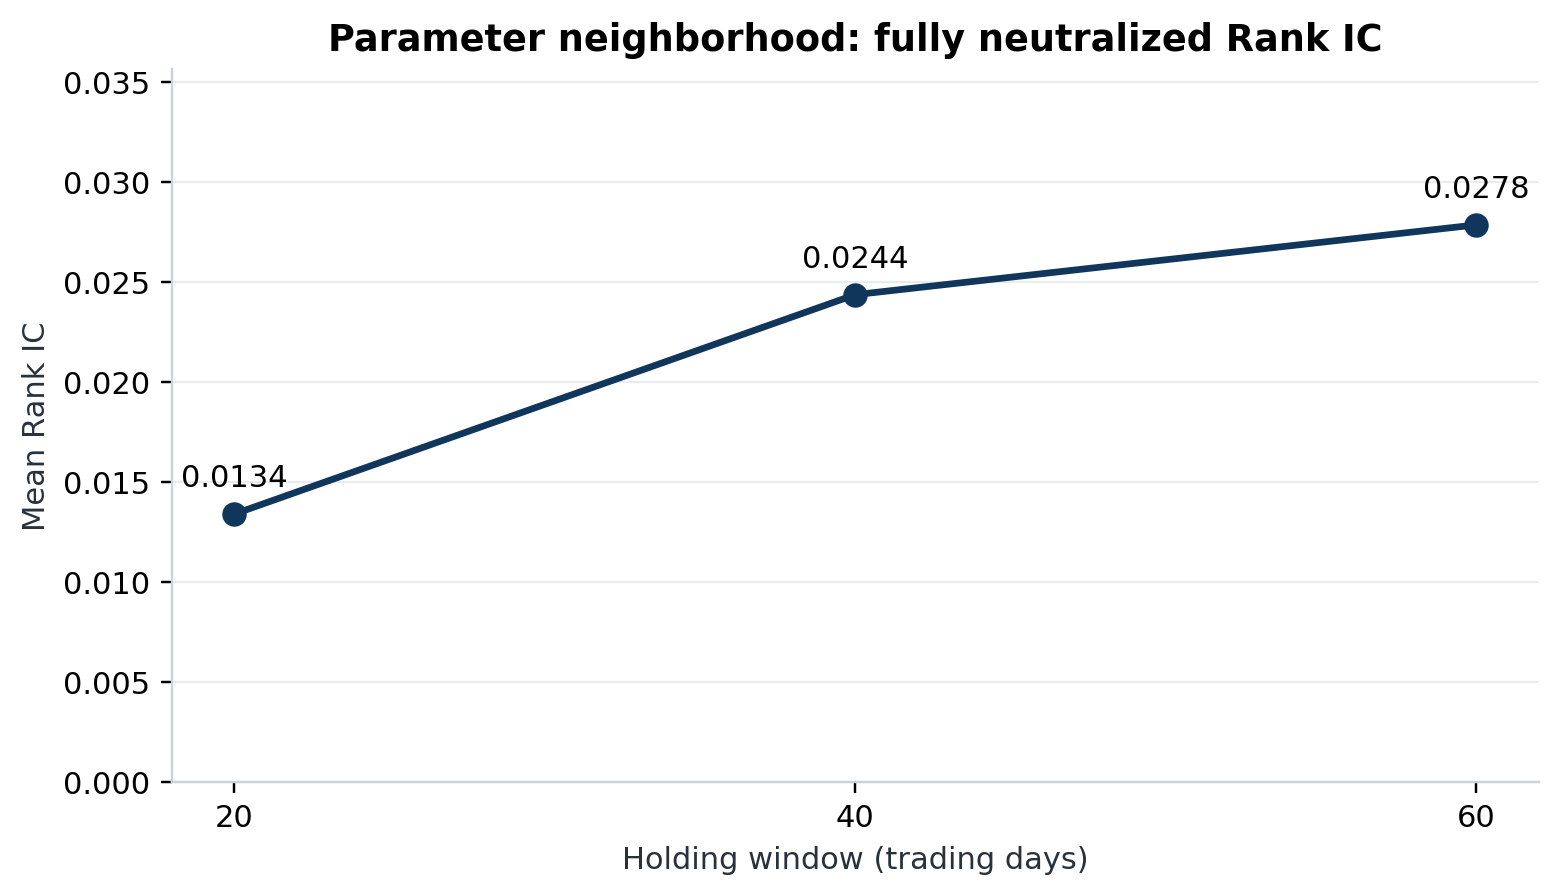
\includegraphics[width=0.78\linewidth]{../results/paper_update/final/figures/hold_neighborhood.png}
  \caption{完整中性化结构化因子在 20/40/60 日持有邻域的平均 Rank IC。数值由确定性结果文件直接生成。}
  \label{fig:hold-neighborhood}
\end{figure}

\subsection{复权与中性化的影响}

表~\ref{tab:ablation} 与图~\ref{fig:ablation} 给出 60 日口径的四档修正。复权使 Rank IC 从 0.0448 上升至 0.0501；仅做市值中性化后为 0.0490；进一步加入行业中性化后降至 0.0278。行业中性化带来约 0.0212 的 IC 降幅，说明原始信号相当一部分与行业构成相关。完整口径仍有正的全样本 IC，但不能把中性化前的更高数字当作纯粹个股选择能力。

\begin{figure}[H]
  \centering
  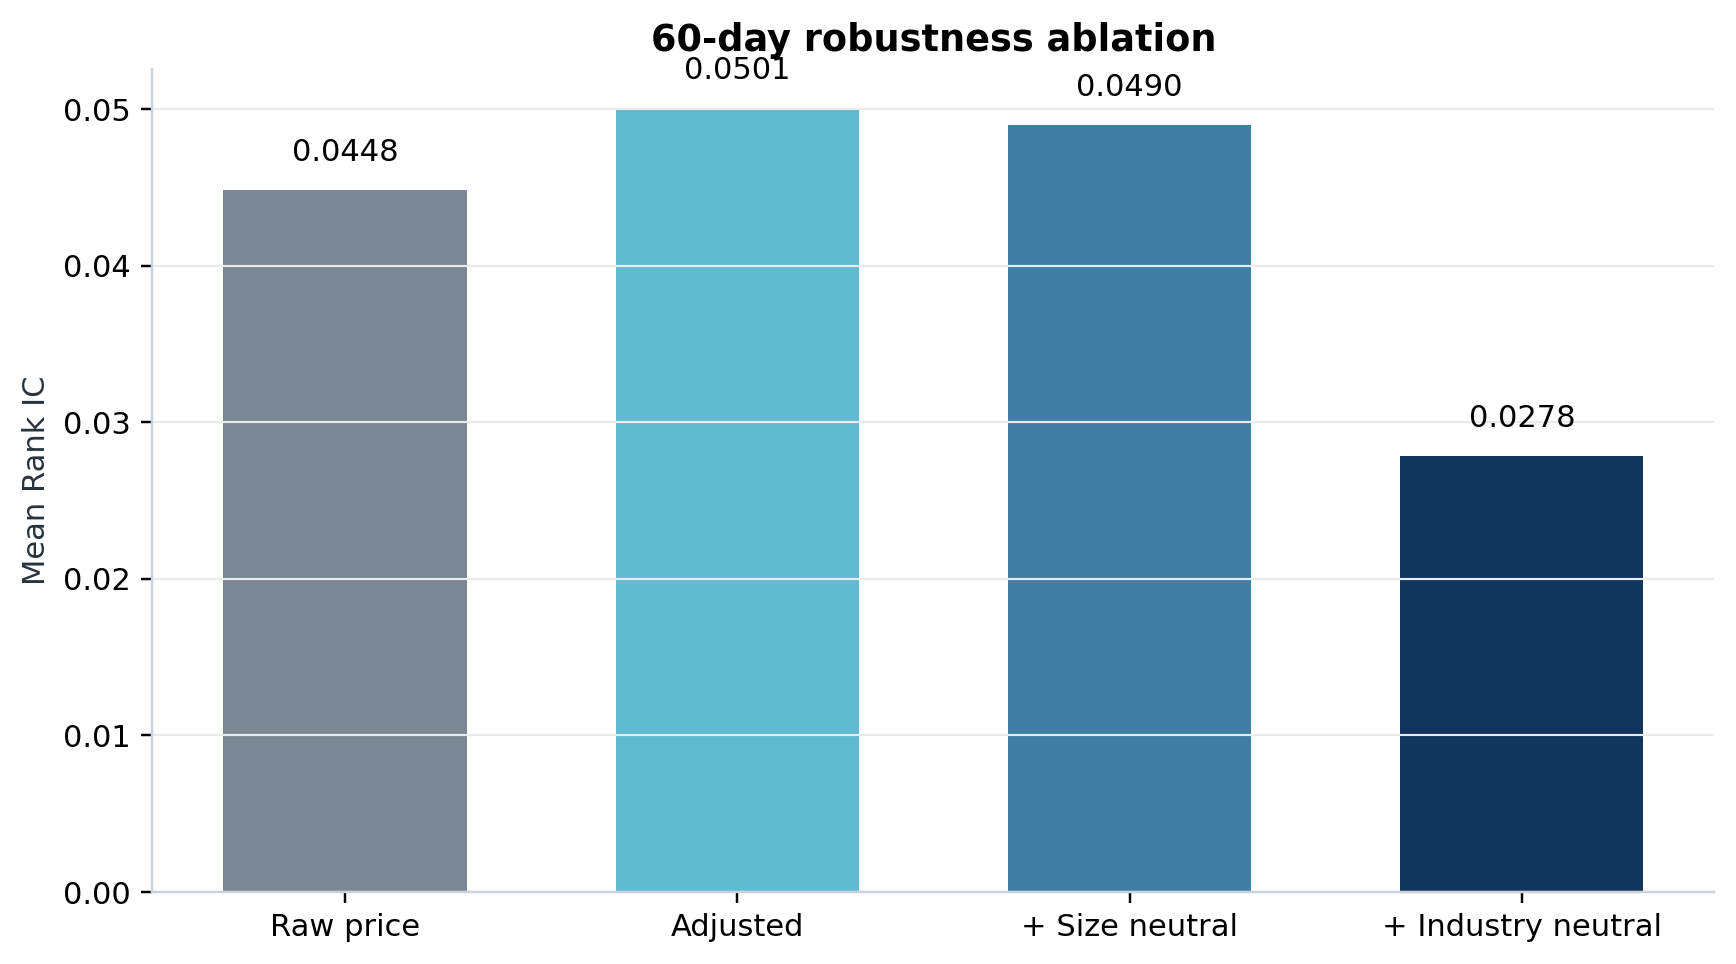
\includegraphics[width=0.82\linewidth]{../results/paper_update/final/figures/ablation_60d.png}
  \caption{60 日结构化对照因子的复权与中性化消融。}
  \label{fig:ablation}
\end{figure}

\subsection{年度稳定性与封存测试}

图~\ref{fig:yearly} 是本文最关键的结果。完整中性化、60 日持有口径在 2019 年和 2020 年的年度 Rank IC 分别为 0.0490 和 0.0467，但 2021 年降至 \TestIC。也就是说，全样本 \FullICSixty 的正 IC 主要来自训练和验证阶段，最终年度没有延续。

\begin{figure}[H]
  \centering
  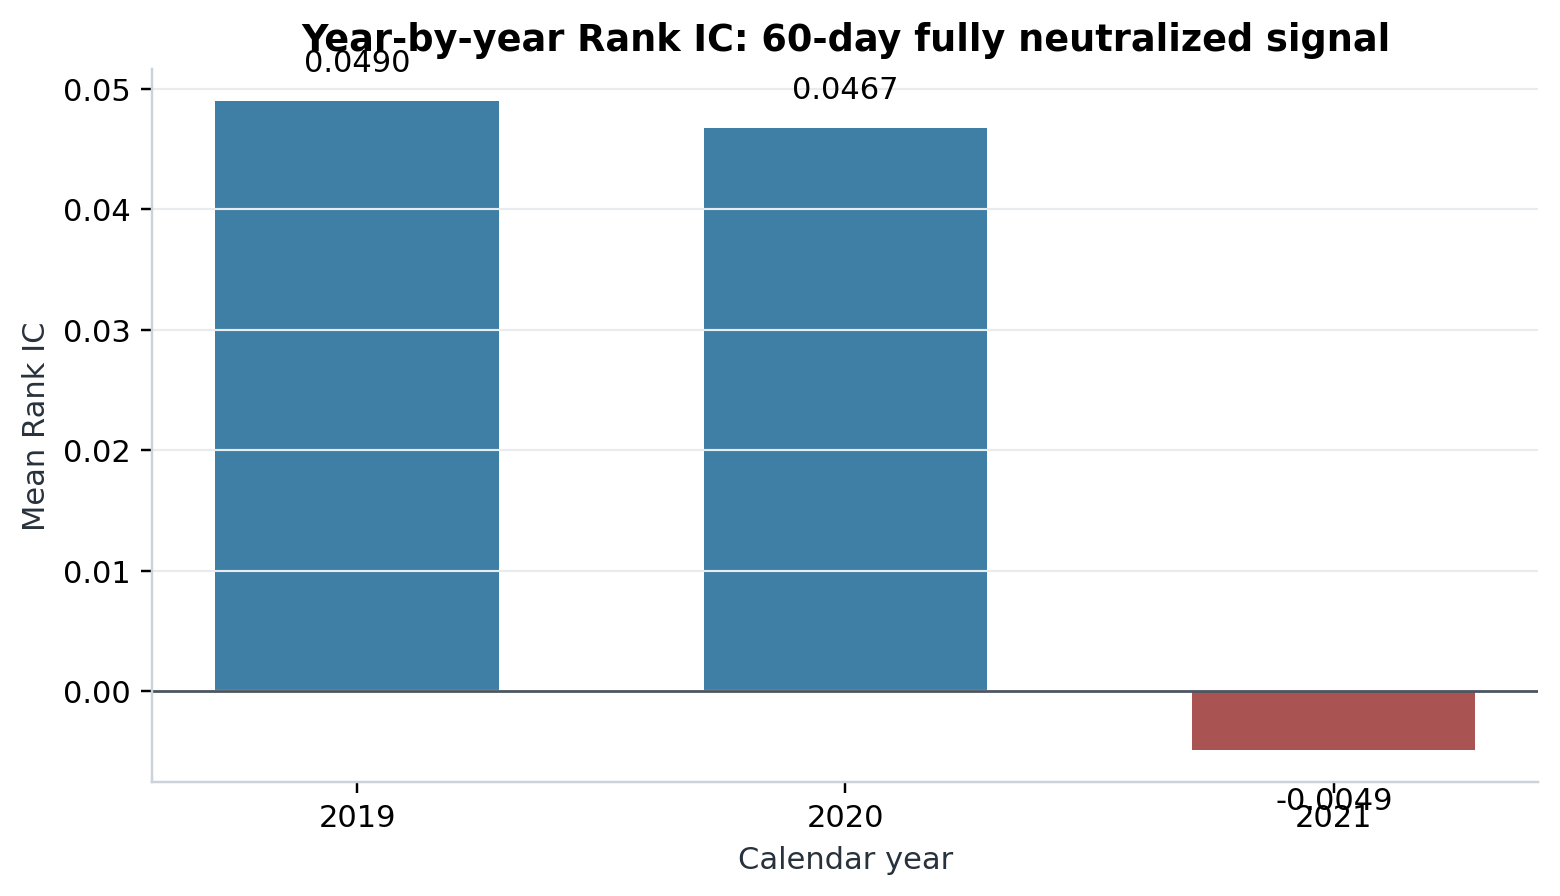
\includegraphics[width=0.78\linewidth]{../results/paper_update/final/figures/yearly_ic.png}
  \caption{60 日完整中性化结构化因子的分年度 Rank IC。2021 年为最终测试年度。}
  \label{fig:yearly}
\end{figure}

这一结果不支持“结构化预告幅度在 2021 年仍有稳定 Alpha”的强结论。它可能反映市场状态变化、事件样本构成变化、信号衰减或开发期偶然性；仅凭三年数据无法区分这些解释。更重要的是，处理组尚未形成，因此不能从结构化因子的失效推导“文本一定有效”。

\subsection{五分组收益}

60 日完整中性化信号的五分组平均 20 日前向收益为：Q1 1.52\%、Q2 1.63\%、Q3 2.24\%、Q4 2.16\%、Q5 2.38\%，Q5--Q1 差约 0.86 个百分点。图~\ref{fig:quantiles} 显示总体从低组向高组上升，但 Q3 高于 Q4，并非严格单调。由于持有窗口重叠、尚未构造真实换手与交易成本序列，本文不把该差值解释为可直接交易的成本后收益。

\begin{figure}[H]
  \centering
  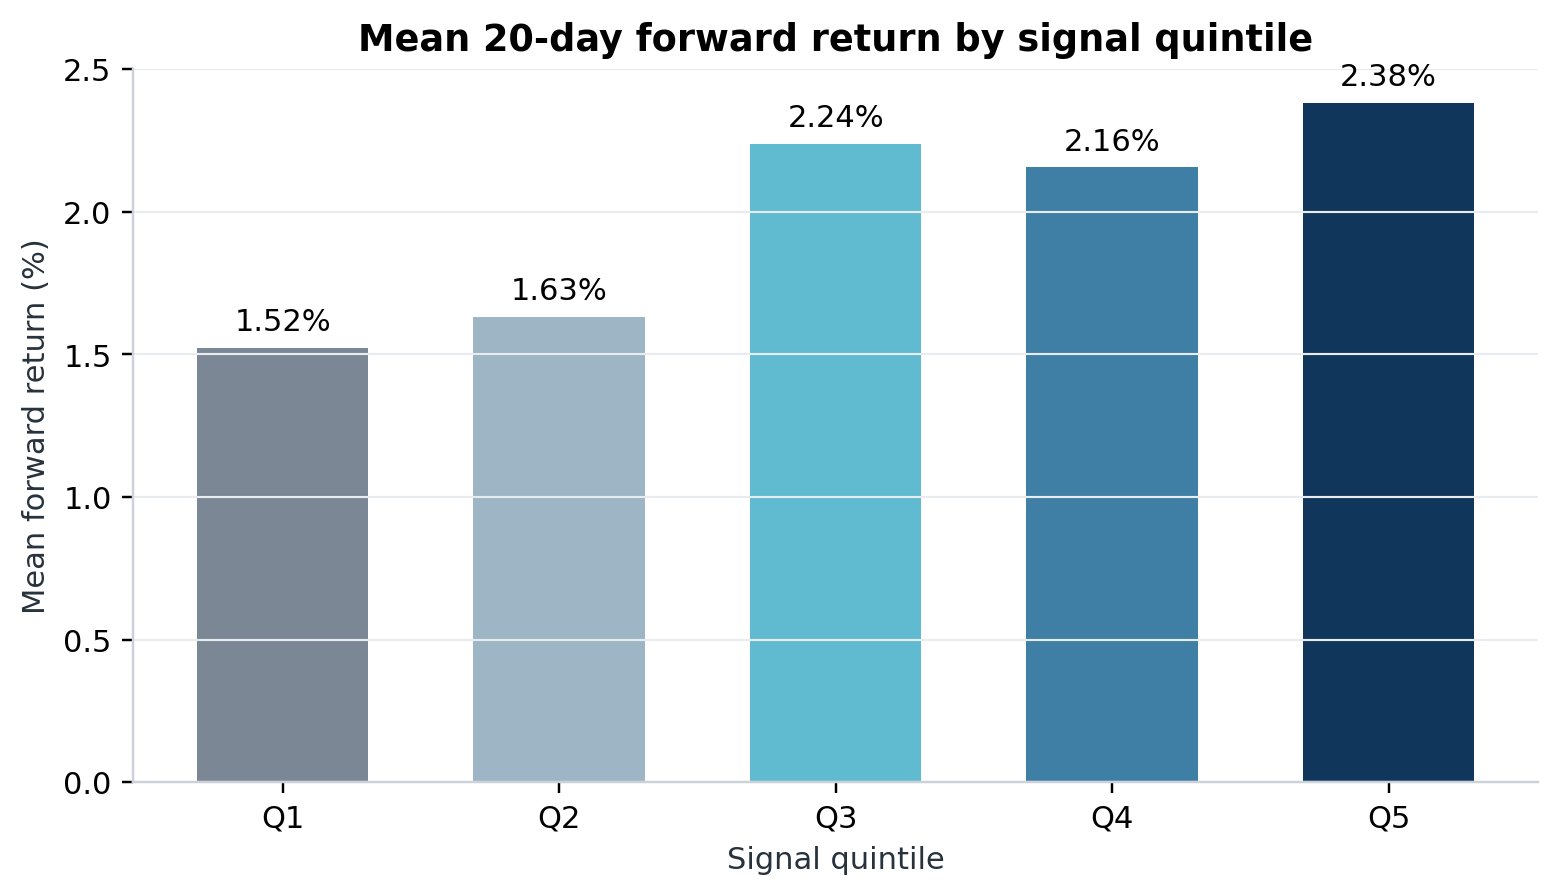
\includegraphics[width=0.78\linewidth]{../results/paper_update/final/figures/quantile_returns.png}
  \caption{60 日完整中性化信号的五分组平均 20 日前向收益。}
  \label{fig:quantiles}
\end{figure}

\subsection{候选漏斗与主问题裁决}

本次记录保留三个代表性候选：结构化预告幅度对照通过确定性校验并完成回测；把未来收益当作当期输入的候选被规则层拒绝；文本增量候选因缺少冻结、可复现的语义特征缓存而不可回测。漏斗为“记录 3 个—通过 1 个—拒绝 1 个—证据不可用 1 个”。

\begin{table}[H]
  \centering
  \caption{候选漏斗与裁决理由}
  \label{tab:funnel}
  \begin{tabular}{p{3.3cm}p{2.2cm}p{7.7cm}}
    \toprule
    候选 & 状态 & 裁决理由 \\
    \midrule
    结构化预告幅度 & 通过 & 字段、PIT 生效日、复权收益与中性化证据齐全，完成确定性回测。 \\
    未来收益反推方向 & 拒绝 & 未来收益只能作为标签，不能成为 $T$ 日因子输入。 \\
    公告文本增量 & 不可用 & 原文已落地，但冻结模型、提示模板、哈希缓存和可复现语义特征缺失。 \\
    \bottomrule
  \end{tabular}
\end{table}

因此，主问题“文本是否在结构化字段之外提供增量 Alpha”在本轮的唯一合规结论是：
\[
  \boxed{\text{insufficient evidence（证据不足）}}
\]
这不是统计意义上的“接受零假设”。它表示处理组尚未被合法构造，增量 IC 不能计算。任何正向或负向文本结论都超出了现有证据。

\section{讨论}\label{sec:discussion}

\subsection{结果如何理解}

结构化预告幅度在 2019--2020 年有较强横截面排序能力，但行业中性化明显削弱信号，且 2021 年转为轻微负值。一个保守解释是：管理层披露的增长幅度在开发期包含信息，但其有效性依赖行业与市场状态，不能视为稳定、跨期的个股 Alpha。本文没有足够证据判断失效来自定价效率提升、样本结构变化还是信号定义本身。

文本处理组缺失也暴露了 LLM 金融研究的关键难点：原始文本“存在”不等于特征“可回测”。可复现的文本因子至少需要固定输入文本、固定模型与提示、输出模式、内容哈希、缓存命中、失败记录和离线重放。否则模型版本漂移或重复 API 调用会让同一公告在不同时间得到不同特征，回测便无法审计。

\subsection{方法论价值}

系统最重要的产出不是某个高 IC 数字，而是三种拒绝能力：
\begin{enumerate}[leftmargin=2.2em,itemsep=1pt,topsep=2pt]
  \item 拒绝未来字段进入因子；
  \item 拒绝用朴素显著性掩盖重叠样本相关；
  \item 拒绝在处理组缺证据时给出想要的结论。
\end{enumerate}
这使“解释”成为因子出生时的结构化假说，而不是看到结果后补写的故事。LLM 可以扩大语义搜索空间，但不能改变数值裁决。

\subsection{与既有工作的关系}

已有 LLM 量化系统往往强调自动生成和策略收益\cite{kou2025}。本文选择更窄的职责分割：生成器可以提出文本语义假说，但代码生成和结果裁决不交给模型。与 AlphaFormer 等符号回归工作\cite{alphaformer2026}相比，本文不追求端到端最优，而是强调每个字段的可得日、每个实验阶段的不可逆性与每个数字的产物来源。两类路线并不冲突：强搜索器可以作为候选来源，但必须服从同一确定性证据链。

\section{有效性威胁与局限}\label{sec:limitations}

\begin{enumerate}[leftmargin=2.2em,itemsep=3pt,topsep=2pt]
  \item \textbf{文本处理组尚未完成。} 原始公告正文虽已导出，但没有冻结、可复现的语义特征缓存，本文无法真正计算增量 IC。这是主结论停在“证据不足”的直接原因。
  \item \textbf{事件期较短。} 可用结构化事件只覆盖 2019 年 6 月至 2021 年末，训练期不足一年，测试期只有一个自然年，统计功效和市场状态覆盖有限。
  \item \textbf{参数邻域包含全时段描述。} 20/40/60 日 JSON 文件均报告 2019--2021 年总体指标及年度拆分，因此总体邻域只能作为事后稳健性描述，不能当作完全未见测试集的调参证据。论文把 2021 年年度值单独作为最终评价，并披露这一限制。
  \item \textbf{研究记录不是第三方预注册。} 不可逆状态机能阻止软件内回退，但本次离线 run record 在结果文件之后生成，缺少外部时间戳，不能独立证明研究者从未提前查看测试结果。
  \item \textbf{交易可实施性不足。} 当前事件脚本未完整加入 ST、停牌、涨跌停、成交容量、冲击成本和组合换手，五分组差不能直接解释为可交易收益。
  \item \textbf{供应商与复权假设。} 单元测试可以证明本项目代码不主动读取未来公告，却不能单独证明供应商日期无误、公告正文未被事后修订或复权序列不存在事后信息。
  \item \textbf{显著性口径有限。} 本文使用滞后 20 阶的 Newey--West 修正处理重叠收益，但未做事件聚类、公司聚类、多重检验或更广泛的自助法检验。
  \item \textbf{样本选择。} 需要增长率上下界的事件才能进入结构化对照，这会排除只披露利润额或定性预告的公司，可能产生覆盖选择偏差。
\end{enumerate}

\section{后续工作}

第一，构建可复现的文本语义缓存：以公告正文哈希为键，冻结模型、提示词与输出 schema，记录失败和重试，确保回测完全离线。第二，在新合同中预注册文本特征、结构化控制、增量定义和显著性检验，并由外部时间戳封存 2021 或更新年份的测试证据。第三，扩展事件历史与滚动样本外窗口，加入行业、规模、预告类型和市场状态分层。第四，补充可交易性过滤、换手与成本模型。第五，在多候选生成时使用固定验证预算和多重检验修正，避免自动化 p-hacking。

\section{结论}

本文没有把“LLM 能生成因子”当作答案，而是把它改写成一个有控制组、处理组和终局状态的增量检验。系统将 LLM 限定在假说与解释空间，将所有数值交给确定性代码，并通过点时间可得性、白名单表达式、Newey--West 修正、日期有序切分和不可逆测试闸门建立证据链。

真实数据结果显示，结构化业绩预告幅度在 2019--2020 年具有正向 Rank IC，但在 2021 年测试段降至 $-0.0049$；行业中性化也显著削弱信号。公告文本原文已经存在，但冻结、可复现的语义特征处理组尚未形成，因此本文不能回答文本增量为正还是为负，最终结论是“证据不足”。

这一结果并非项目失败。相反，一个可信的因子智能体必须有能力说“不知道”，并能指出缺少哪一条证据。本文证明的不是某个稳定 Alpha，而是一套让 LLM 提出假说、让代码做出裁决、让每个结论都能追溯到确定性产物的研究方法。

\section*{可复现性与产物映射}
\addcontentsline{toc}{section}{可复现性与产物映射}

本论文数字由脚本从既有确定性 JSON 结果生成，不重新调用 LLM，也不重新估计因子：
\begin{verbatim}
python scripts/build_final_paper_assets.py
cd paper && latexmk -xelatex -interaction=nonstopmode main.tex
\end{verbatim}

关键产物如下：
\begin{longtable}{p{5.0cm}p{8.4cm}}
  \toprule
  产物 & 用途 \\
  \midrule
  \raggedright\path{results/workflow/forecast_hold_20.json}（另含 40/60 日） & 参数邻域、消融、年度 IC、Newey--West $t$ 与五分组收益的确定性来源。 \\
  \raggedright\path{results/workflow/research_run_record.json} & 冻结合同、候选漏斗、验证预算、测试拆封与终局状态。 \\
  \raggedright\path{results/paper_update/final/manifest.json} & 论文数据版本、源文件 SHA-256、输出清单与数值不经 LLM 的声明。 \\
  \raggedright\path{results/paper_update/final/} 下的 CSV & 论文表格的机器可读版本。 \\
  \raggedright\path{results/paper_update/final/figures/} & 从 CSV/JSON 同源生成的论文图。 \\
  \bottomrule
\end{longtable}

\addcontentsline{toc}{section}{参考文献}
\begin{thebibliography}{99}
  \bibitem{fama1973}
  Fama, E. F., \& MacBeth, J. D. (1973).
  Risk, return, and equilibrium: Empirical tests.
  \emph{Journal of Political Economy}, 81(3), 607--636.
  doi:10.1086/260061.

  \bibitem{newey1987}
  Newey, W. K., \& West, K. D. (1987).
  A simple, positive semi-definite, heteroskedasticity and autocorrelation consistent covariance matrix.
  \emph{Econometrica}, 55(3), 703--708.
  doi:10.2307/1913610.

  \bibitem{mclean2016}
  McLean, R. D., \& Pontiff, J. (2016).
  Does academic research destroy stock return predictability?
  \emph{The Journal of Finance}, 71(1), 5--32.
  doi:10.1111/jofi.12365.

  \bibitem{gkx2020}
  Gu, S., Kelly, B., \& Xiu, D. (2020).
  Empirical asset pricing via machine learning.
  \emph{The Review of Financial Studies}, 33(5), 2223--2273.
  doi:10.1093/rfs/hhaa009.

  \bibitem{kou2025}
  Kou, Z., Yu, H., Luo, J., Peng, J., Li, X., Liu, C., Dai, J., Chen, L., Han, S., \& Guo, Y. (2025).
  Automate strategy finding with LLM in quant investment.
  \emph{Findings of the Association for Computational Linguistics: EMNLP 2025}, 18517--18533.
  doi:10.18653/v1/2025.findings-emnlp.1005.

  \bibitem{alphaformer2026}
  Huang, H., Peng, J., Ding, Z., Li, P., \& Chen, T. (2026).
  AlphaFormer: End-to-end symbolic regression of alpha factors with Transformers.
  \emph{Proceedings of Machine Learning Research}, 328, 61--82.
\end{thebibliography}

\end{document}
